\documentclass{article}
\usepackage{graphicx} 
\usepackage[hidelinks]{hyperref}
\usepackage{url}

\title{\fontsize{19}{10}\textbf{SMB Attack diagnostics \& recovery - A Wireshark Analysis and Firewall}}

\author{\textbf{Abdullah Mohammad Aref}}
\date{\textbf{July 2025}}

\begin{document}

\maketitle

\begin{flushleft}
    
    \textbf{Sample capture:}
    \url{https://wiki.wireshark.org/uploads/__moin_import__/attachments/SampleCaptures/smb-browser-elections.pcapng}
    
\end{flushleft}

\tableofcontents

\section{Introduction}

In this sample capture, a master browser is responsible for several tasks like:
\begin{itemize}
    \item Tracking all clients in this network
    \item  Respond to requests from clients
\end{itemize}
When a client sends a request and the master browser doesn't respond, it's assumed by the client that there is no master browser, and an election starts where all clients participate to choose the new master browser. 


\section{problem}

One of the clients has his firewall configured incorrectly, causing the messages coming from UDP port 138 to be blocked. This makes the client think that there is no master browser, and it starts the elections, which significantly slows the network because all clients stop working and focus on the elections. Then the clients realize that there is a master browser, so they get back to work, but the client that initiated this election still thinks that there is no master browser, and it keeps starting an election infinity. This slows the network and causes processes to stop working; Therefore, in decreasing efficiency.

\section{analysis}
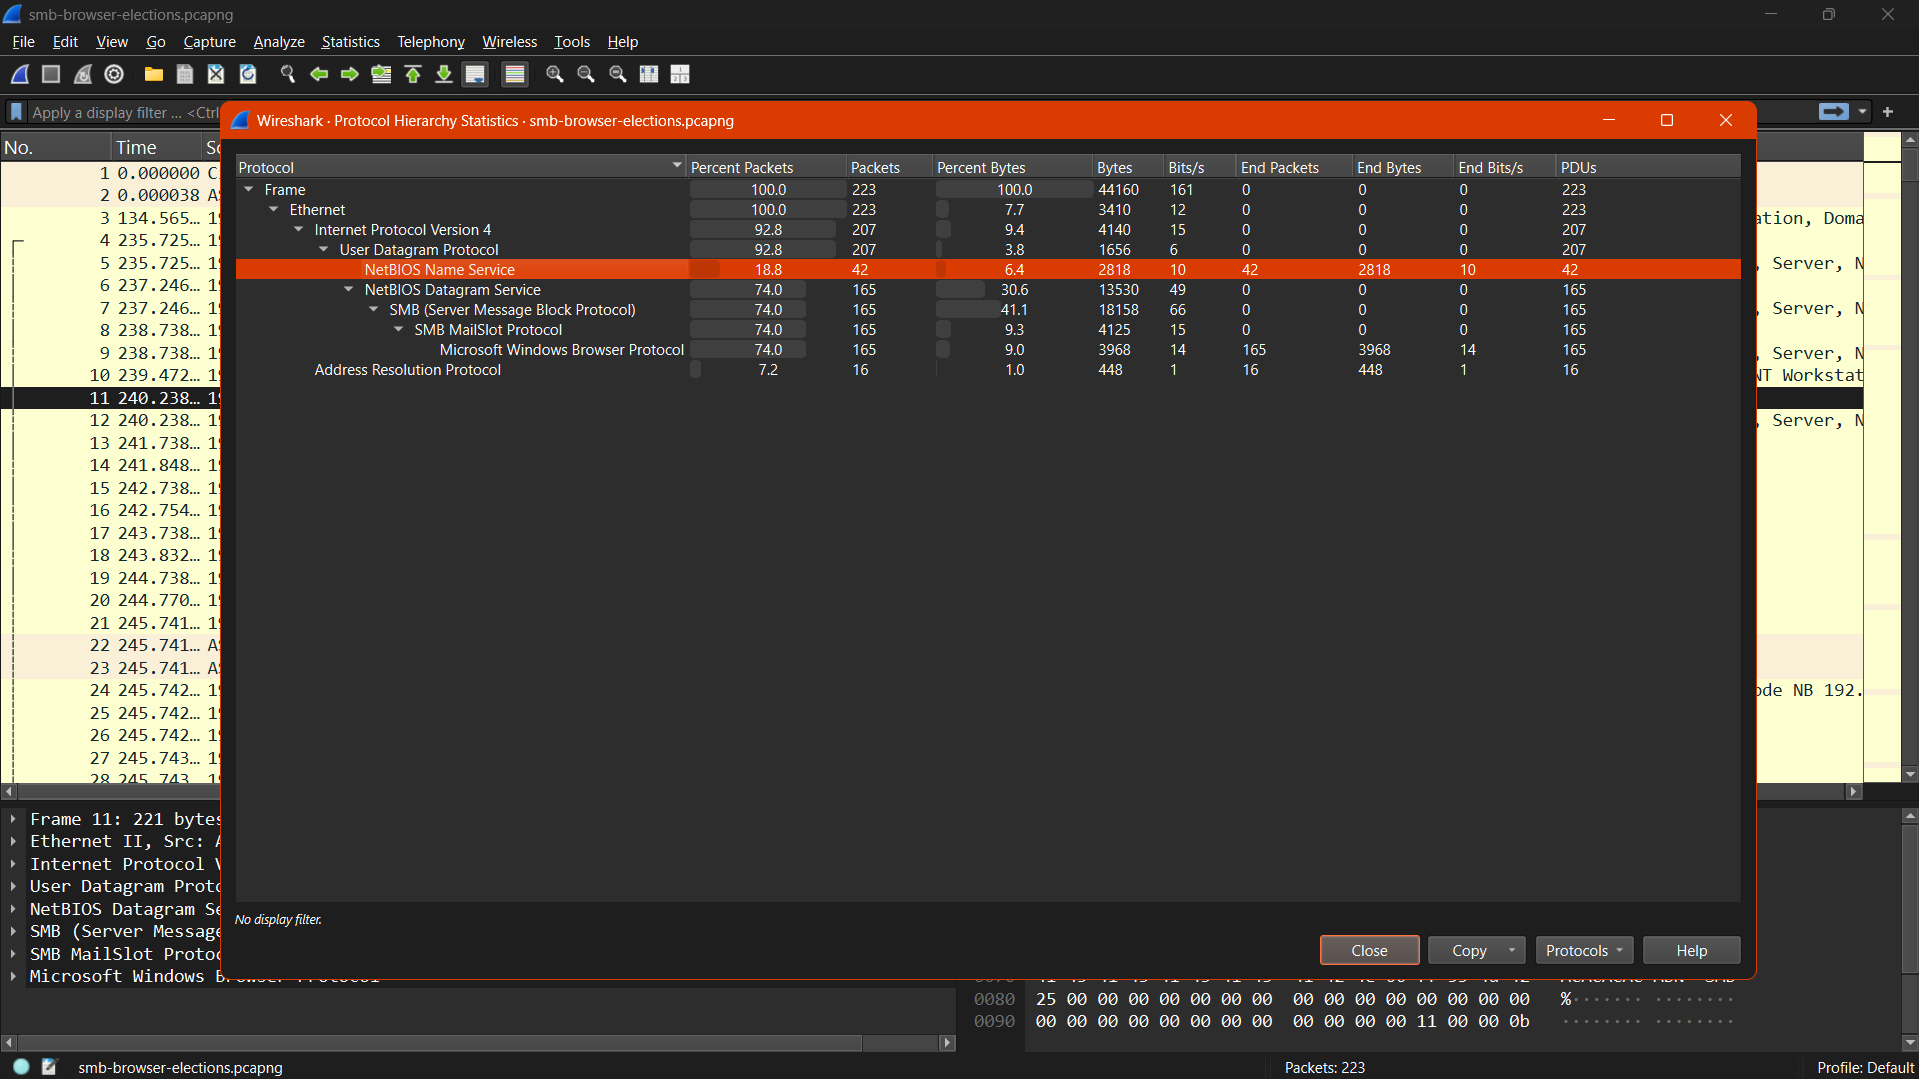
\includegraphics[width=1\textwidth]{protocol hyerarchy}
Going to the protocol hierarchy statistics, we can see that in total, this file consists of 223 captured packets over an Ethernet connection. 207 of these packets are IPv4 UDP packets. The rest are ARP packets. From those 207 UDP packets, there are 42 packets from the NetBios Name service, but the remaining 165 are from the SMB(server message block protocol). This shows how most of the packets have been blocked due to this issue. This information is important for pinpointing and confirming the source of the problem. We can also conclude that the client might have been under an SMB attack.

A filter to show the first 56 packets was applied, as a common pattern is happening, so this removes extra noise

We can see two sources: 192.168.123.1, 192.168.123.2. So we update the filter to only packets with these source IP addresses. We got the following result:

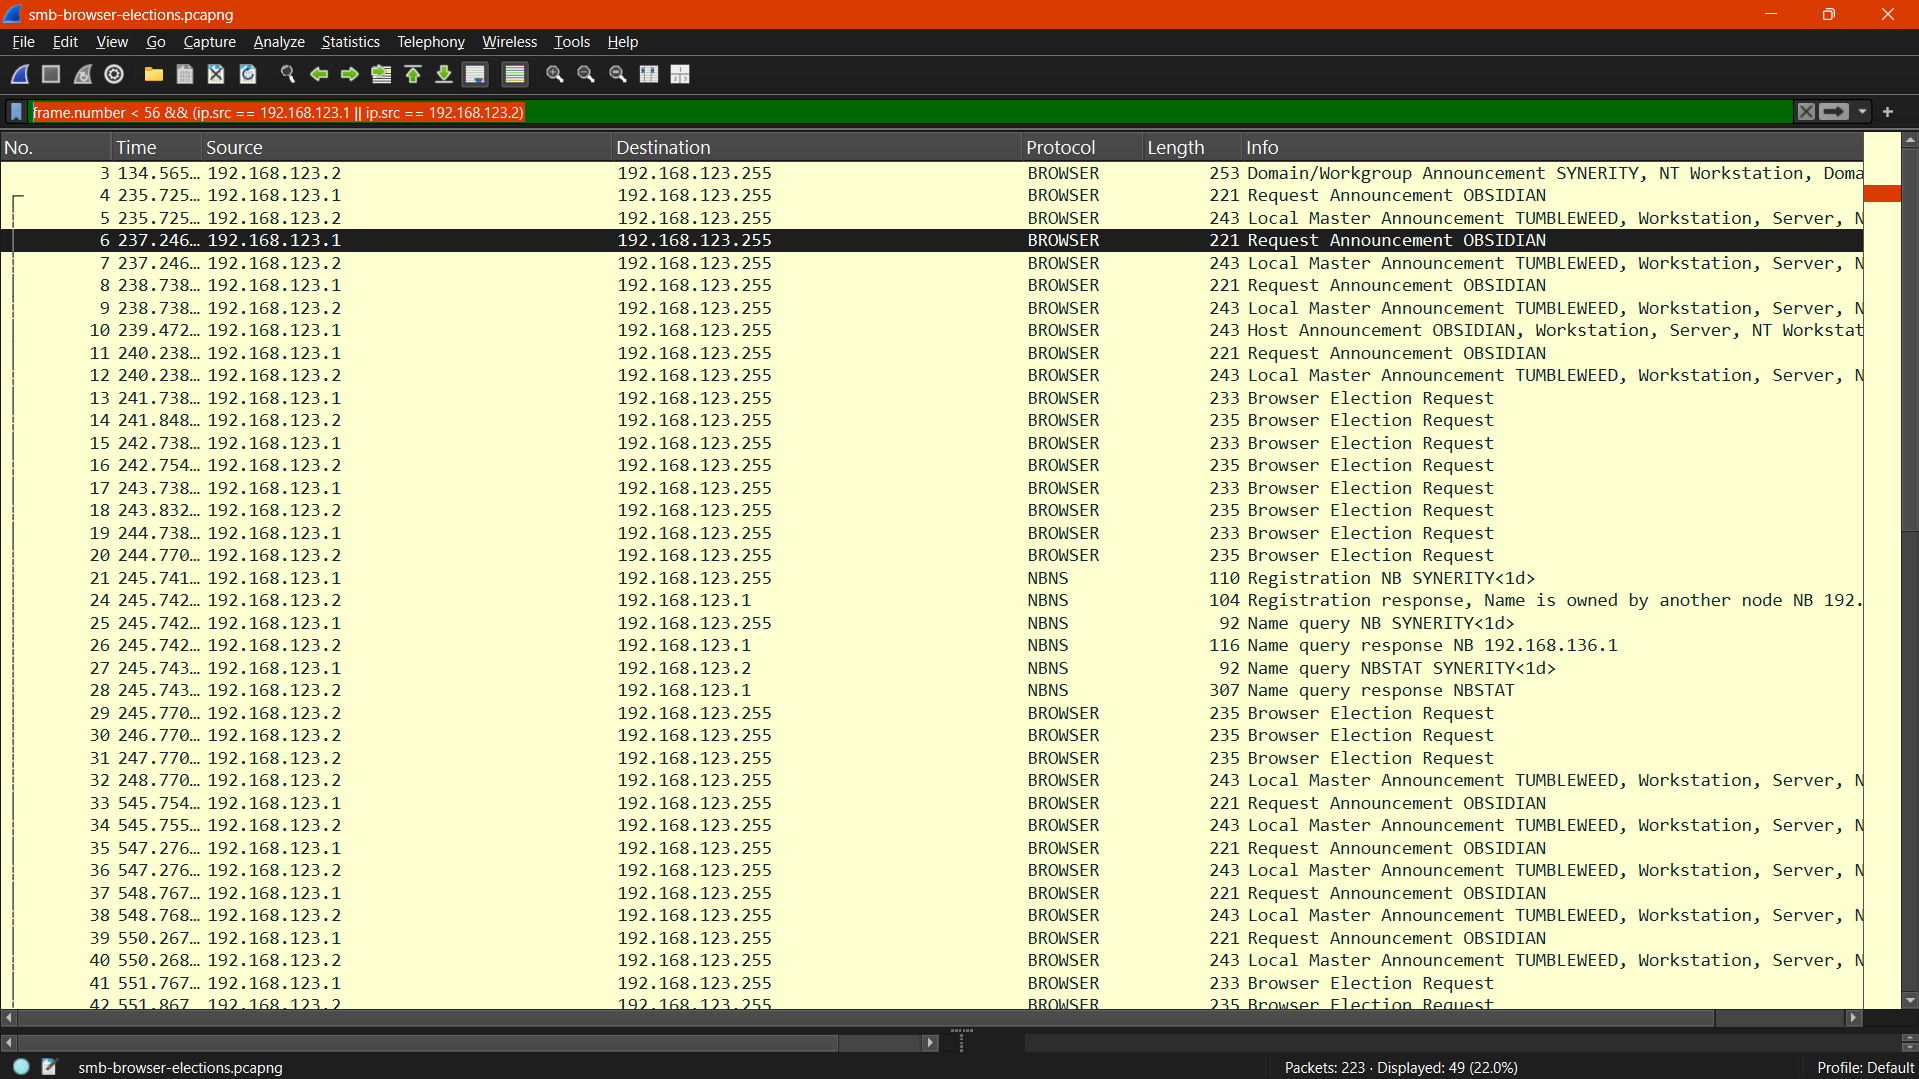
\includegraphics[width=1\textwidth]{filter}

This shows that "192.168.123.1" is requesting an "OBSIDIAN" announcement in packets 4, 6, 8, 10, 11, etc. But 192.168.123.2 is only announcing "TUMBLEWEED, Workstation, Server, NT Workstation, Potential Browser, Master Browser". This shows that the client is "192.168.123.1" and the master browser is "192.168.123.2".

When we enter "UDP.port == 138" nothing changes, so we know that all these packets are on port 138 as it was described in the sample capture description.

Now to see if "192.168.123.1" is receiving messages from port 138, the following filter is applied: "ip.dst == 192.168.123.1 \&\& !(ip.src == 192.168.123.2)". And the expected outcome has occurred (No packets were shown)

Finally, entering the "smb" filter will show exactly 165 packets (the same number of packets that we saw in the protocol hierarchy smb). This shows that it is most likely that the client was a victim to a smb attack that changes a firewall setting to block all UDP messages on port 138.




\section{solution}

Now that we know the problem and its source, we can solve this issue by applying the following firewall rules:

\begin{itemize}
    \item Firstly, we need to reverse the changes of the SMB attack for the attacked client(192.168.123.1), by setting a PERMIT rule that allows received UDP protocol messages on port 138 
    \item  Secondly, to prevent this attack from happening to any of the clients again, we need to go to all these clients and block all messages from external sources that are received on UDP protocol on port 138 to prevent external requests, which can lead to attacks.
    
\end{itemize}

\section{conclusions}

This sample capture has demonstrated the importance of a firewall and its effects on the network. As one misconfigured firewall rule can ruin an entire network configuration and cause problems for other computers.

\section{References}

Samplecaptures - wireshark wiki (no date). Available at: https://wiki.wireshark.org/samplecaptures (Accessed: 3 July 2025).

\end{document}
